%%%%%%%%%%%%%%%%%%%%%%%%%%%%%%%%%%%%%%%%%
% baposter Landscape Poster
% LaTeX Template
% Version 1.0 (11/06/13)
%
% baposter Class Created by:
% Brian Amberg (baposter@brian-amberg.de)
%
% License:
% CC BY-NC-SA 3.0 (http://creativecommons.org/licenses/by-nc-sa/3.0/)
%
%%%%%%%%%%%%%%%%%%%%%%%%%%%%%%%%%%%%%%%%%

%----------------------------------------------------------------------------------------
% PACKAGES AND OTHER DOCUMENT CONFIGURATIONS
%----------------------------------------------------------------------------------------

\documentclass[landscape,a0paper,fontscale=0.285]{baposter} % Adjust font scale/size

\usepackage{graphicx} % Required for including images
\graphicspath{{figs/}} % Directory in which figures are stored
\usepackage{float}

\usepackage{amsmath} % For typesetting math
\usepackage{amssymb} % Adds new symbols to be used in math mode
\usepackage{mathtools}

\usepackage[numbers]{natbib}
\usepackage{caption}
\usepackage{subcaption}
%\usepackage{subfigure}
\usepackage{booktabs} % Top and bottom rules for tables
\usepackage{enumitem} % Used to reduce itemize/enumerate spacing
\usepackage{palatino} % Use the Palatino font
\usepackage[font=small,labelfont=bf]{caption} % Required for specifying captions to tables and figures

\usepackage{multicol} % Required for multiple columns
\setlength{\columnsep}{1.5em} % Slightly increase the space between columns
\setlength{\columnseprule}{0mm} % No horizontal rule between columns

\newcommand{\compresslist}{ % Define a command to reduce spacing within itemize enumerate environments, this is used right after \begin{itemize} or \begin{enumerate}
\setlength{\itemsep}{1pt}
\setlength{\parskip}{0pt}
\setlength{\parsep}{0pt}
}

\definecolor{lightblue}{rgb}{0.145,0.6666,1} % Defines color of content box headers

\begin{document}

\begin{poster} {
headerborder=closed, % Adds a border around the header of content boxes
colspacing=1em, % Column spacing
bgColorOne=white, % Background color for the gradient on the left side of the poster
bgColorTwo=white, % Background color for the gradient on the right side of the poster
borderColor=lightblue, % Border color
headerColorOne=black, % Background color for the header in the content boxes (left side)
headerColorTwo=lightblue, % Background color for the header in the content boxes (right side)
headerFontColor=white, % Text color for the header text in the content boxes
boxColorOne=white, % Background color of the content boxes
textborder=roundedleft, % Format of the border around content boxes, can be: none, bars, coils, triangles, rectangle, rounded, roundedsmall, roundedright or faded
eyecatcher=true, % Set to false for ignoring the left logo in the title and move the title left
headerheight=0.1\textheight, % Height of the header
headershape=roundedright, % Specify the rounded corner in the content box headers, can be: rectangle, small-rounded, roundedright, roundedleft or rounded
headerfont=\Large\bf\textsc, % Large, bold and sans serif font in the headers of content boxes
%textfont={\setlength{\parindent}{1.5em}}, % Uncomment for paragraph indentation
linewidth=2pt % Width of the border lines around content boxes
}
%----------------------------------------------------------------------------------------
% TITLE SECTION
%----------------------------------------------------------------------------------------
%
{
\includegraphics[height=6.5em]{logo_berkeley.jpg}} % First university/lab logo on the left
{\bf\textit{\LARGE Robust inference on the causal effects of stochastic
    interventions in two-phased vaccine efficacy
    trials}\vspace{0.01em}} % Poster title
{\textbf{Nima Hejazi, David Benkeser, and Mark van der Laan} \\
  \textit{Graduate Group in Biostatistics \& Department of Statistics,
    University of California, Berkeley} \\
  \textit{Department of Biostatistics and Bioinformatics, Emory University}}
    % Author names and institution
{
\includegraphics[height=6.5em]{logo_emory.jpg}} % Second university/lab logo on the right

%-------------------------------------------------------------------------------
% OVERVIEW
%-------------------------------------------------------------------------------

\headerbox{Overview \& Motivations}{name=overview,column=0,row=0}{

\begin{itemize}\compresslist
\setlength\itemsep{0.75em}
\item We consider estimating the effect of a stochastic intervention in vaccine
  trials with two-phase sampling of the treatment.
\item We present robust, efficient estimators of the mean counterfactual outcome
  under a stochastic intervention.
\item The proposed estimators are asymptotically normal with a variance
  estimator based on the efficient influence function.
\item Our \texttt{txshift} \texttt{R} package~\cite{hejazi2019txshift}
  implements these estimators and leverages state-of-the-art machine learning in
  the procedure.
\item Our \texttt{haldensify} \texttt{R} package~\cite{hejazi2019haldensify}
  estimates a generalized propensity score (a conditional
  density) via highly adaptive lasso (HAL).
\end{itemize}
\vspace{0.75cm} % When there are two boxes, some whitespace may need to be added
                % if the one on the right has more content
}

%-------------------------------------------------------------------------------
% INTRODUCTION
%-------------------------------------------------------------------------------

\headerbox{HIV Vaccine Efficacy Trials}
{name=introduction,column=1,row=0,bottomaligned=overview}{

\begin{itemize}\compresslist
\setlength\itemsep{0.5em}
\item \underline{Question}: How does HIV infection risk vary across shifts of an
  immunogenic response profile in a trial's vaccine arm.
\item Analysis of data from the HIV Vaccine Trials Network 505 efficacy trial,
  as in \cite{janes2017higher}:
  \begin{itemize}
    \itemsep0.25pt
    \item RCT with $n = 2504$; only $n = 189$ from vaccine arm in second-stage
      sample.
    \item Background covariates $(W)$: sex, age, BMI, behavioral HIV risk score.
    \item Treatment $(A)$: immunogenic response profiles, post-vaccination.
    \item Outcome $(Y)$: HIV-1 infection status at week 28 of trial.
    \item All individuals with HIV-1 infections by week 28 in second-stage
      sample.
  \end{itemize}
\item \underline{Goal}: Develop a ranking of immunogenic responses as study
  endpoints for future HIV-1 vaccine efficacy trials.
\end{itemize}
}

%-------------------------------------------------------------------------------
% Methodology cont.
%-------------------------------------------------------------------------------

\headerbox{Efficient Corrections for Two-Phase Sampling}{name=results,
  column=2,span=2,row=0}{

\vspace{-0.35em}
\begin{itemize}
  \itemsep-2pt
\item In the HVTN 505 HIV-1 trial, immunogenic responses $A$ are sequenced for
  infected individuals and a matched subset of controls, making
  \textbf{$O = (W, \Delta, \Delta A, Y)$} the observed data structure.
  \vspace{-0.25em}
  \begin{itemize}
    \itemsep0pt
    \item $\Delta \in \{0, 1\}$ is the sampling mechanism introduced by
      two-phase sampling, under which the observed immunogenic response
      ($\Delta A$) is arbitrarily set to $0$ when unobserved.
    \item Given $V \coloneqq (W, Y)$, we assume that $\Delta \sim
      \text{Bern}(\pi_0(V))$.
  \end{itemize}
\item The IPCW-TMLE~\cite{rose2011targeted2sd} estimates the target parameter by
  incorporating inverse probability weights (of sampling) in the estimation of
  the outcome regression and generalized propensity score.
\item Efficiency improvements are attainable by constructing estimators based on
  the augmented EIF:
  \begin{equation*}
    D(P_0)(o) = \frac{\Delta}{\pi(v)} D^F(P_0^X)(X) - \left(1 -
      \frac{\Delta}{\pi(v)}\right)\mathbb{E}(D^F(P_0^X)(x) \mid \Delta = 1,
      V = v)
  \end{equation*}
\item This augmentation allows the construction of estimators that
  \vspace{-0.5em}
  \begin{itemize}
    \itemsep0pt
    \item achieve the efficiency bound for the class of regular asymptotically
      linear estimators;
    \item are \textit{multiply robust}, with consistency of parameter estimates
      when one of $\{g, Q\}$ and one of $\{\pi_0(V), \mathbb{E}_0(D^F(P_0^X)(X)
      \mid \Delta = 1, V)\}$ are consistently estimated;
    \item allow valid statistical inference even when $\pi_0$ is estimated
      nonparametrically.
  \end{itemize}
\end{itemize}
}

%-------------------------------------------------------------------------------
% REFERENCES
%-------------------------------------------------------------------------------

\headerbox{\small References}{name=references,column=2,above=bottom}{
\renewcommand{\section}[2]{\vskip 0.05em} % remove "References" section title
\tiny{ % Reduce the font size in this block
\setlength{\bibsep}{0.1pt}
\bibliographystyle{plainnat}
%\nocite{*} % Insert publications even if they are not cited in the poster
\bibliography{2019_jsm}
\compresslist
\vspace{-0.7em}
}
}

%-------------------------------------------------------------------------------
% CONTACT
%-------------------------------------------------------------------------------

\headerbox{\small Contact Information}{name=ack,column=3,aligned=references,above=bottom}{
% This block is as tall as the references block
\begin{itemize}
  \itemsep0.25pt
  \item \textbf{N.~Hejazi}, Graduate Group in Biostatistics, UC Berkeley,
    \texttt{nhejazi@berkeley.edu}
  \item \textbf{D.~Benkeser}: Asst.~Prof.~of Biostatistics, Emory University,
    \texttt{benkeser@emory.edu}
  \item \textbf{M.~van der Laan}, Prof.~of Biostatistics, UC Berkeley,
    \texttt{laan@berkeley.edu}
\end{itemize}
}

%-------------------------------------------------------------------------------
% CONCLUSION
%-------------------------------------------------------------------------------

\headerbox{Numerical Study \& Results}
{name=conclusion,column=2,span=2,row=0,below=results,above=references}{

\vspace{-1.25em}
\begin{figure}[H]\label{fig:sim_results}
  \begin{subfigure}[b]{0.48\textwidth}
    \centering
    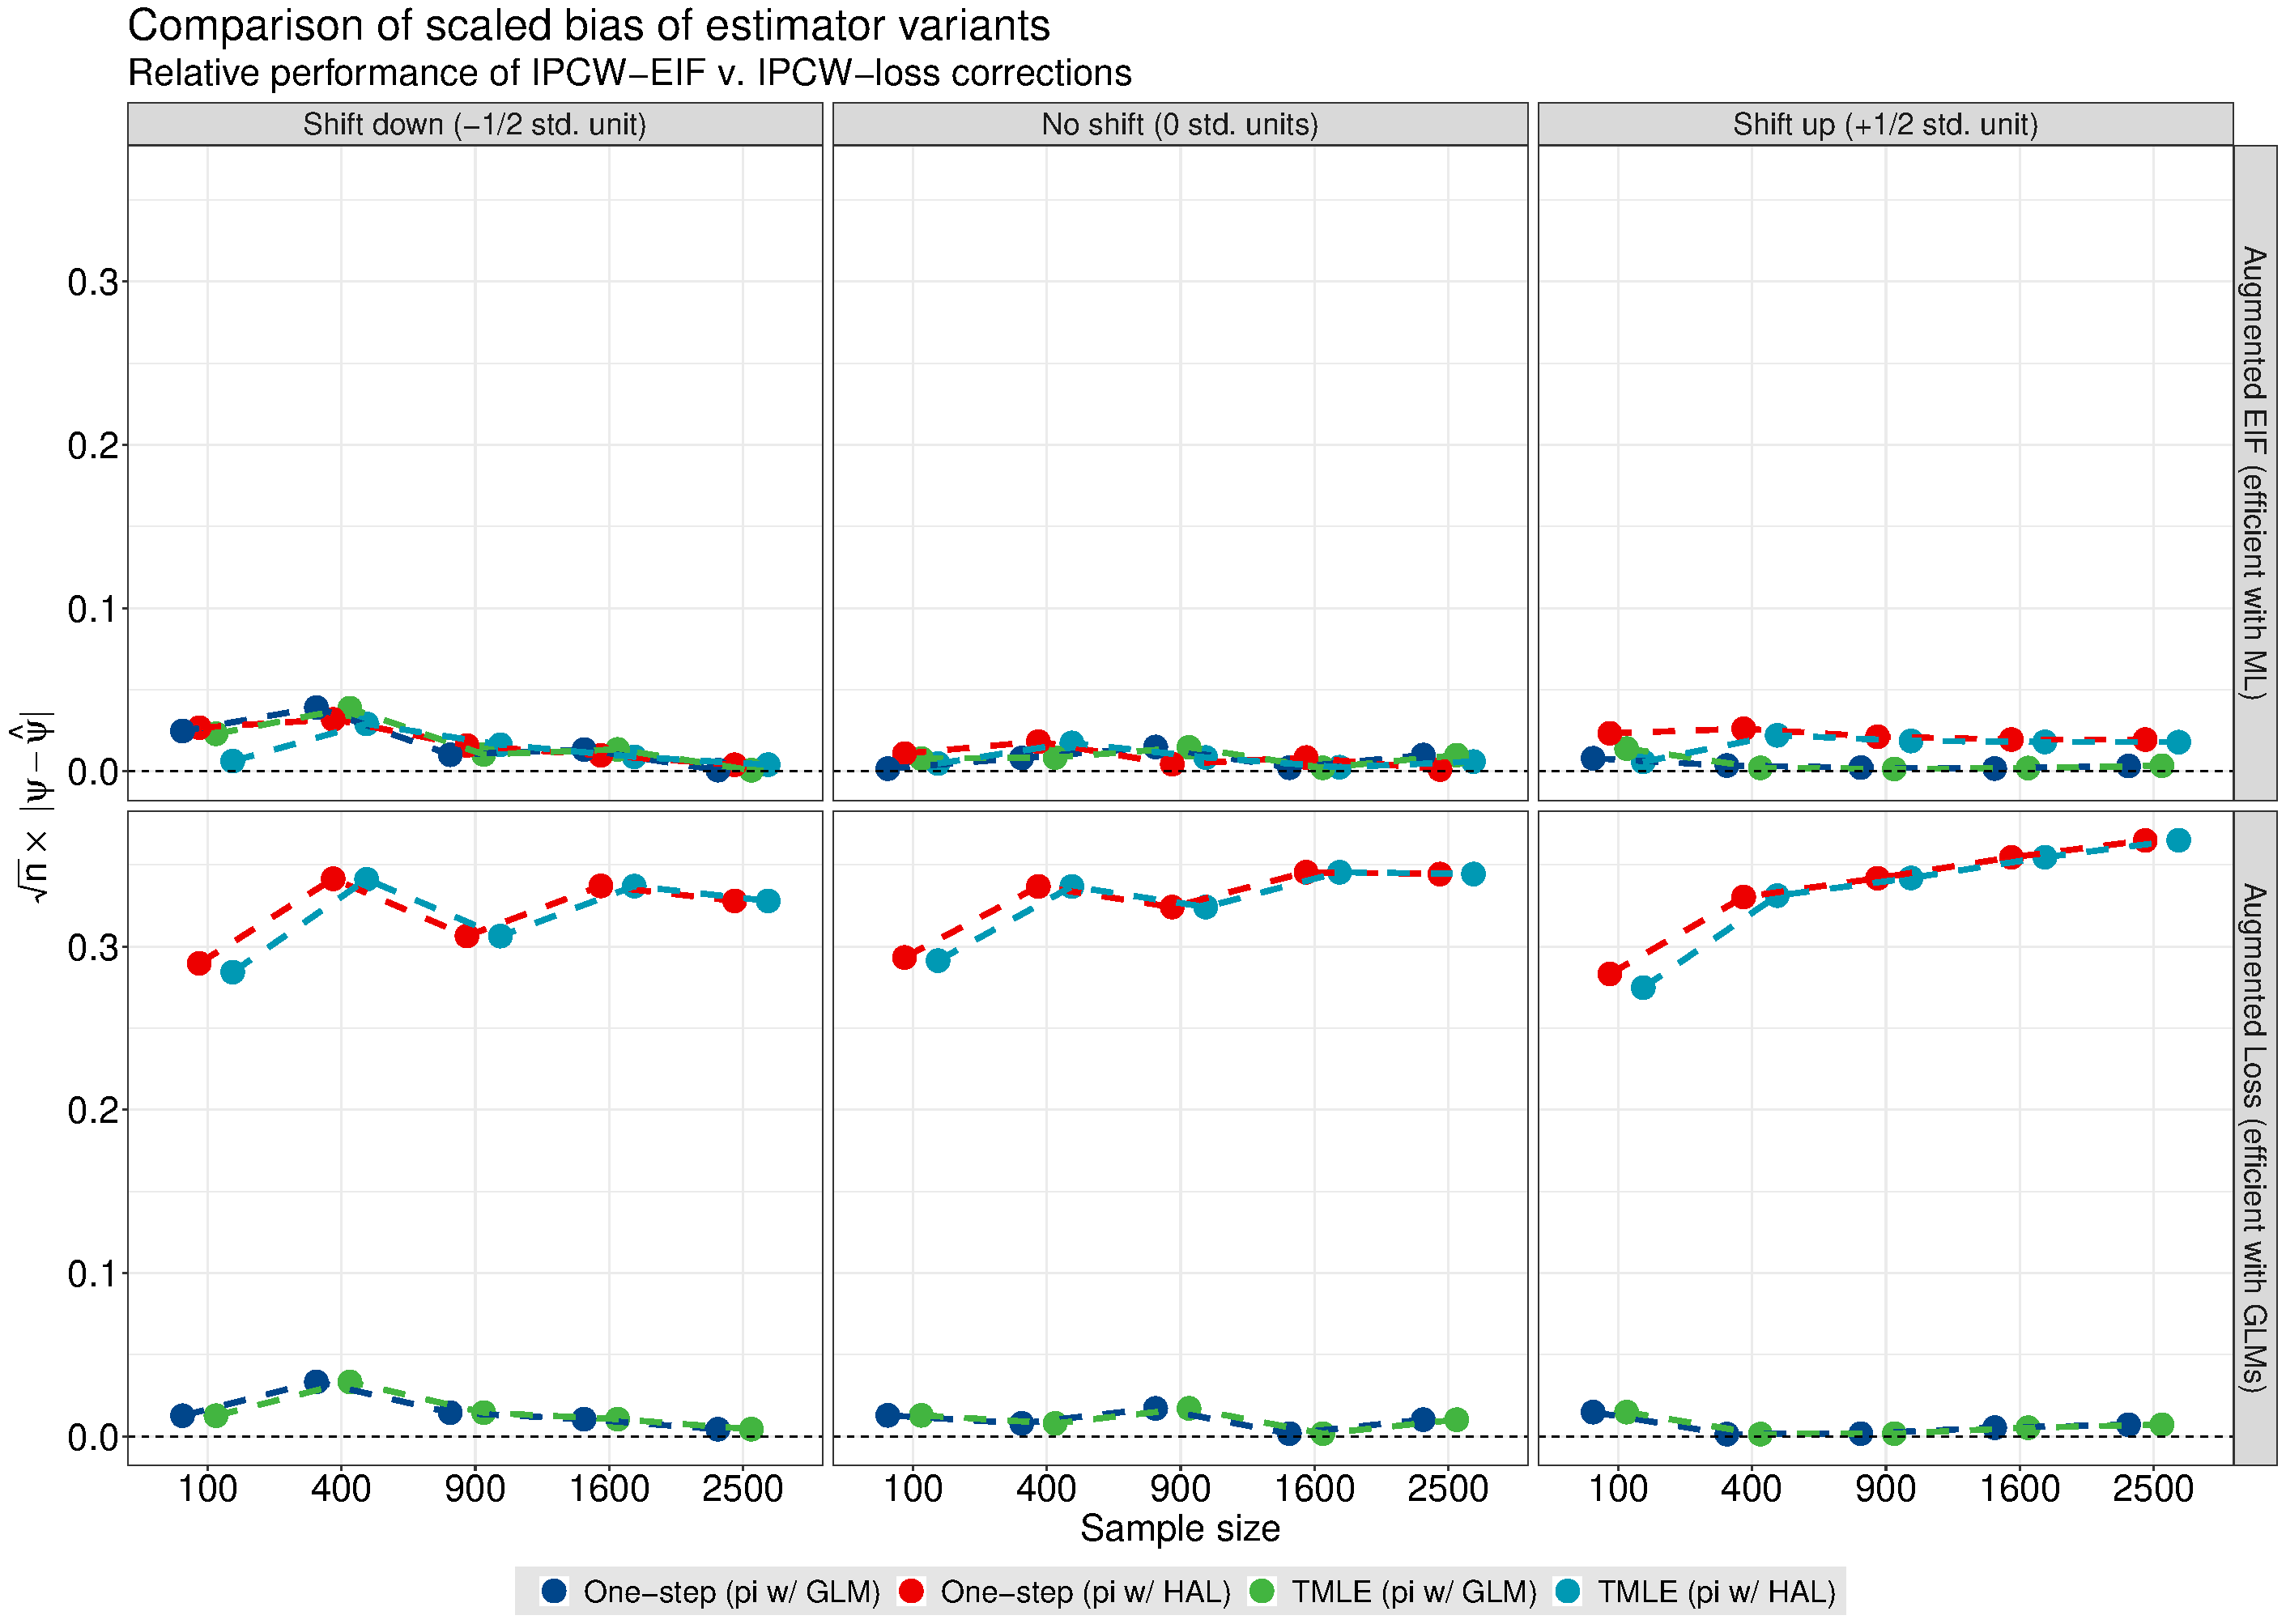
\includegraphics[scale=0.16]{bias_scaled}
    \caption{Most estimator variants unbiased in large samples; inefficient
      variants with HAL fail to converge.}
    \label{fig:bias}
  \end{subfigure}%
  \hspace{1.5em}
  \begin{subfigure}[b]{0.48\textwidth}
    \centering
    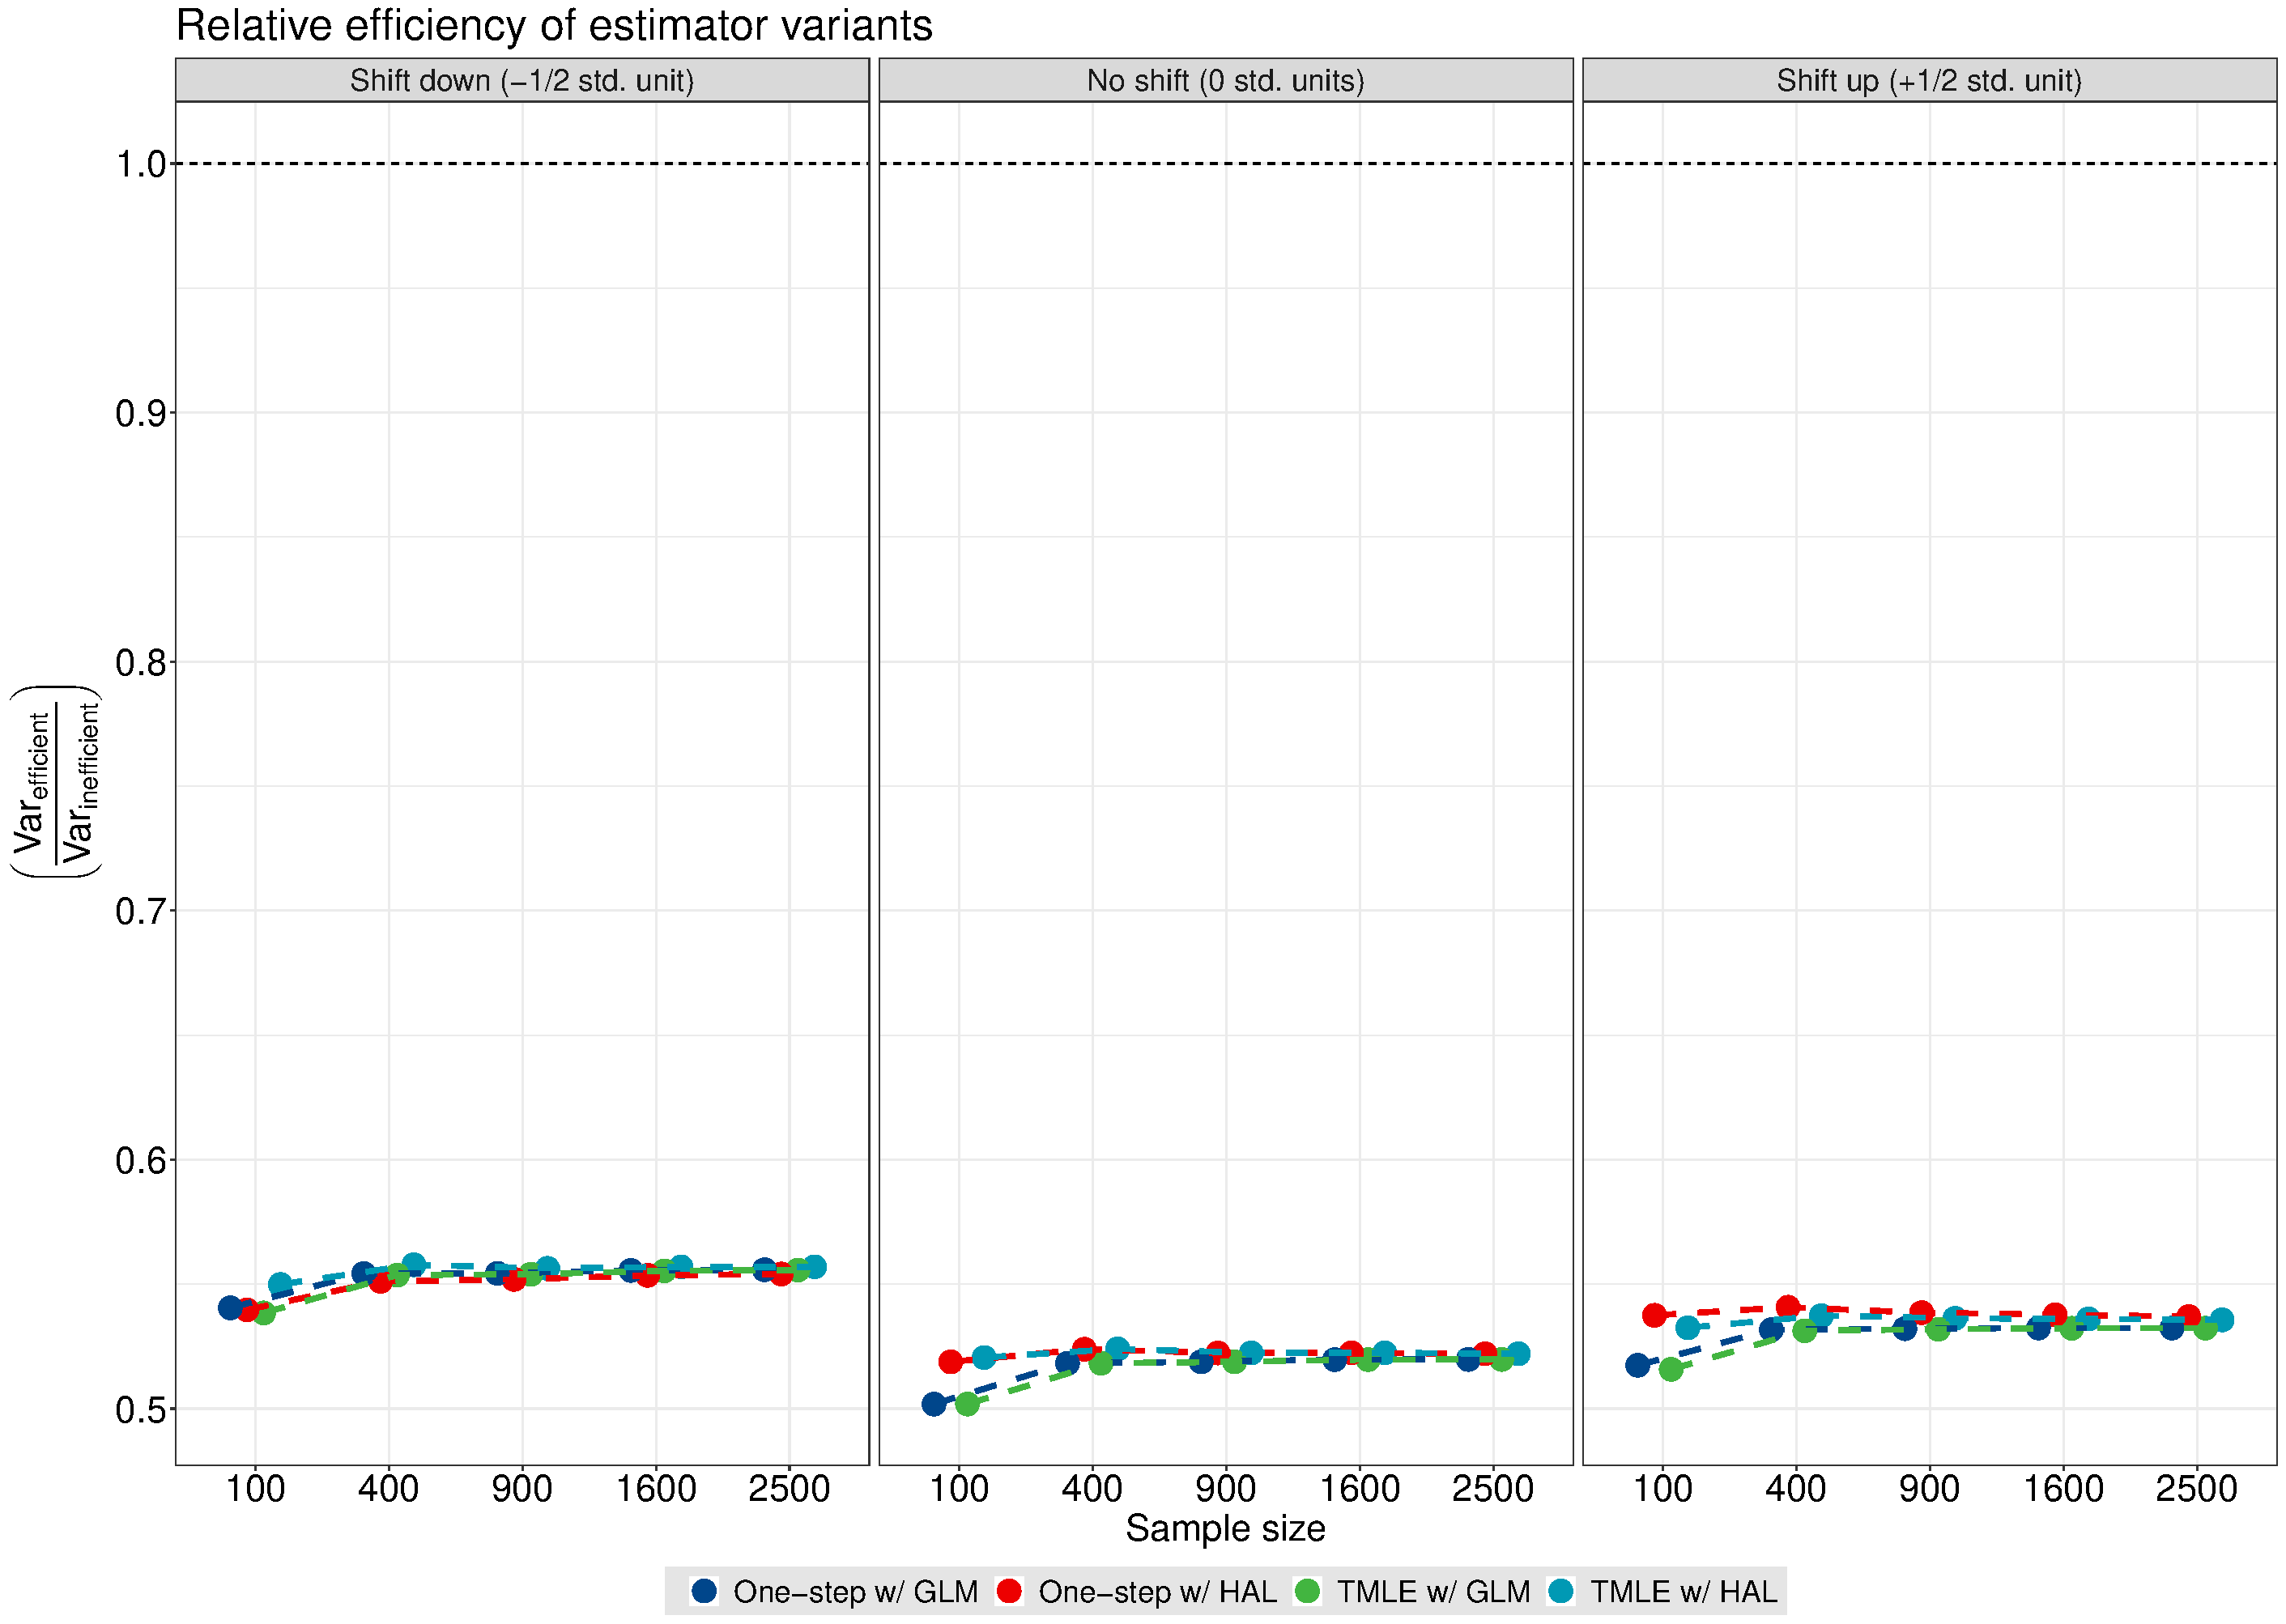
\includegraphics[scale=0.16]{rel_eff}
    \caption{Fitting $\pi$ with HAL or GLM, efficient estimators and simpler
      variants show comparable relative efficiency.}
    \label{fig:efficiency}
  \end{subfigure}
\end{figure}
}

%-------------------------------------------------------------------------------
% METHODS
%-------------------------------------------------------------------------------

\headerbox{The Effect of a Stochastic Treatment Regime}{name=method,column=0,
  span=2,below=overview,bottomaligned=references}{
% This block's bottom aligns with the bottom of the conclusion block

\begin{itemize}
  \itemsep0.75pt
  \item Consider $X = (W, A, Y) \sim P_0^X \in \mathcal{M}$, where $W$ is a set
    of baseline covariates, $A$ a treatment, and $Y$ an outcome of interest,
    with no assumptions placed on the statistical model $\mathcal{M}$.
  \item Consider a shift of the treatment $d(A, W) = A + \delta$ for a given
    shift $\delta$. To protect against violations of the positivity assumption,
    make the shifting mechanism a function of the observed data, where $u(w)$ is
    the maximum shift supported in the observed data:
    \[ d(a, w) =
       \begin{cases}
         a + \delta, & a + \delta < u(w) \\
         a, & \text{otherwise}
       \end{cases}
    \]
  \item The causal parameter has been shown to be identified by a functional of
    the observed data~\cite{munoz2012population}:
    \begin{equation*}
      \Psi(P_0^X) = \mathbb{E}_{\text{P}_0}{\overline{Q}(d(A, W), W)},
    \end{equation*}
    where $\overline{Q}(d(A, W), W)$ is the conditional mean of the outcome
    given $A = d(A,W)$ and $W$.
  \item The efficient influence function (EIF) of $\Psi$ relative to the
    nonparametric model $\mathcal{M}$ is
    \begin{equation*}
      D^F(P_0^X)(x) = H(a, w)({y - \overline{Q}(a, w)}) +
        \overline{Q}(d(a, w), w) - \Psi(P_0^X)(x),
    \end{equation*}
    where the auxiliary covariate term $H(a,w)$ may be expressed as
    \begin{equation*}
      H(a,w) = \mathbb{I}(a < u(w)) \frac{g(a - \delta \mid w)}{g(a \mid w)}
        + \mathbb{I}(a \geq u(w) - \delta).
    \end{equation*}
%We obtain Wald-style inference via the limiting distribution:
%$\sqrt{n}(\Psi_n - \Psi) \to N(0, \text{Var}(D(P_0)))$.
\end{itemize}
}

%-------------------------------------------------------------------------------
\end{poster}
\end{document}
